%%%%%%%%%%%%%%%%%%%%%%%%%%%%%%%%%%%%%%%%%%%%%%%%%%%%%%%%%%%%%%%%%%%%%%%%%%%%%%
%%%%%% Generic paper template 
%%%%%% - by, Swapnil V. Patil (svp -at- cs.cmu)
%%%%%% - UPDATED: 1.1.11
%%%%%% 
%%%%%%%%%%%%%%%%%%%%%%%%%%%%%%%%%%%%%%%%%%%%%%%%%%%%%%%%%%%%%%%%%%%%%%%%%%%%%%

\documentclass[pdftex,twoside,twocolumn,10pt,letterpaper]{article}
% -OR-
%\documentclass[pdftex,twoside,article,10pt,letterpaper]{article}

%%%%%% Page formatting
%%%%%% 
\pdfpagewidth 8.5in
\pdfpageheight 11in

\setlength\topmargin{0.0in}             %%%%%% Margins (top, even-/odd- pages)
\setlength\oddsidemargin{0.0in}         %%%%%% - default=1in (i.e., 1+x)
\setlength\evensidemargin{0.0in}

\setlength\headheight{0.0in}            %%%%%% Header info
\setlength\headsep{0in}

\setlength\textwidth{6.5in}             %%%%%% Main text body 
\setlength\textheight{9.0in}
\setlength\topskip{0in}
\setlength\footskip{0.25in}
\setlength\columnsep{0.25in}

%%%%%% Increase the textwidth by X, but keep the same relative placing
%%%%%% 
\advance\textwidth by 0in               %%%%%% X
\advance\oddsidemargin by -0in          %%%%%% -X/2
\advance\evensidemargin by -0in         %%%%%% -X/2

%%%%%% Decrease the margins by X
%%%%%% 
\advance\textwidth by 0in               %%%%%% 2X
\advance\oddsidemargin by -0in          %%%%%% -X
\advance\evensidemargin by -0in         %%%%%% -X

%%%%%% Paragraph spacing, widows/orphans 
%%%%%%
\setlength\parindent{0.10in}            %%%%%% Paragraph spacing 
\setlength\parskip{0.03in}

\clubpenalty=1000                       %%%%%% No orphans
\widowpenalty=1000                      %%%%%% No widows
\interfootnotelinepenalty=10000         %%%%%% No split footnotes

%%%%%% Formatting setup for captions, sections and subsections 
%%%%%%
\makeatletter  % Allow the use of @ in command names
\long\def\@makecaption#1#2{%
  \vskip\abovecaptionskip
  \sbox\@tempboxa{{\captionfonts #1: #2}}%
  \ifdim \wd\@tempboxa >\hsize
    {\captionfonts #1: #2\par}
  \else
    \hbox to\hsize{\hfil\box\@tempboxa\hfil}%
  \fi
  \vskip\belowcaptionskip}

%%%%%% Captions
%%%%%%
\ifx\abovecaptionskip\@undefined
  \newskip\abovecaptionskip
  \newskip\belowcaptionskip
\fi
\abovecaptionskip=0.5\baselineskip
\belowcaptionskip=-0.5\baselineskip
\long\def\@makecaption#1#2{%
  \vskip\abovecaptionskip
  \sbox\@tempboxa{\small\textbf{#1} -- {#2}}%
  \ifdim \wd\@tempboxa >\hsize
    {\small\textbf{#1} -- {#2}\par}
  \else
    \global \@minipagefalse
    \hb@xt@\hsize{\hfil\box\@tempboxa\hfil}%
  \fi
  \vskip\belowcaptionskip}

%%%%%% Section, subsection and subsubsection formatting 
%%%%%%
\renewcommand\section{\@startsection 
  {section}{1}{0mm}%                        % name, level, indent
  {-2ex \@plus -1ex \@minus -2ex}%        % X + Y - space above SECTITLE
  {0.5ex \@plus.2ex}%                       % for spacing after SECTITLE 
  %{\sf\bfseries\fontsize{18}{18}\selectfont}
  {\normalfont\bfseries\fontsize{13}{13}\selectfont}
}
\renewcommand\subsection{\@startsection 
  {subsection}{2}{0mm}%                     % name, level, indent
  {-2ex \@plus -1ex \@minus -2ex}%        % X + Y - space above SECTITLE
  {0.5ex \@plus.2ex}%                       % for spacing after SECTITLE 
  %{\sf\bfseries\fontsize{16}{16}\selectfont}
  {\normalfont\bfseries\fontsize{11}{11}\selectfont}
}
\renewcommand\subsubsection{\@startsection 
  {subsubsection}{3}{0mm}%                  % name, level, indent
  {-2ex \@plus -1ex \@minus -2.2ex}%        % X + Y - space above SECTITLE
  {-1ex \@plus.2ex}%                        % for spacing after SECTITLE 
  %{\sf\bfseries\fontsize{14}{14}\selectfont}
  {\normalfont\bfseries\fontsize{11}{11}\selectfont}
}
\makeatother

%%%%%% Fonts and typesetting 
%%%%%%
\usepackage[T1]{fontenc}
\usepackage{textcomp}
\usepackage{mathptmx}           %%%%% Times + Times-like math symbols
\usepackage{courier}
\usepackage[scaled=0.92]{helvet}
%%%%%% Uncomment these lines to use a GARAMOND font (if available)
%\renewcommand{\rmdefault}{ugm} %%%%%% UGM Garamond
%\usepackage[adobe-utopia]{mathdesign}
%%%%%%

%%%%%% Bibliography using bibtex 
%%%%%%
\usepackage[numbers,sort&compress, square]{natbib}   %%%%% BIBTEX
%\usepackage{natbib}   %%%%% BIBTEX
%\bibpunct{[}{]}{;}{a}{}{,}

%%%%%% Tables and figures
%%%%%%
\usepackage[pdftex]{graphicx}           %%%%% PDFLATEX (for PDF figures)
\usepackage{lscape}                     %%%%% Landscape rotation
\usepackage{rotating}                   %%%%% ?
\usepackage{booktabs}                   %%%%% ?
\usepackage[table]{xcolor}              %%%%% Colors in tables

%%%%%% Misc
%%%%%%
\usepackage{verbatim}                   %%%%% Block comments (\begin{comment}) 
\usepackage{color}                      %%%%% Graphics
\usepackage{thumbpdf}                   %%%%% ?
\usepackage{url}                        %%%%% URL formatting

%%%%%% Proof-reading (increase the spacing; default: singlespacing)
%%%%%%
\usepackage{setspace}
\singlespacing
% -OR-
%\onehalfspacing
% -OR-
%\doublespacing

%%%%%%%%%%%%%%%%%%%%%%%%%%%%%%%%%%%%%%%%%%%%%%%%%%%%%%%%%%%%%%%%%%%%%%%%%%%%%%
%%%%%% Additional useful packages that need special style files

%%%%%% Lists
%%%%%%
%\usepackage{enumitem}
%\setlist{itemsep=0pt,parsep=0pt}        %%%%%% More compact lists

%%%%%% For "To appear/appeared" in text on title page
%%%%%% 
%\usepackage[absolute]{textpos}
%\newcommand{\ToAppear}{%
%\begin{textblock*}{\textwidth}(0.95in,0.4in)
%\begin{flushright}
    %\noindent{\fbox{\textsf{Under submission---please do not redistribute.}}}
    %  --OR--
%    \noindent{\fbox{\textsf{Working draft---please do not redistribute.}}}
    %  --OR--
    %\noindent{\small To appear in \textit{Proceedings of the XYZ}\\
    %\noindent{\small \textit{Conference (XYZ'99)}, City, State, Month Year}}
%\end{flushright}
%\end{textblock*}
%}

%%%%%% Misc
%\usepackage{soul}
%%%%%%%%%%%%%%%%%%%%%%%%%%%%%%%%%%%%%%%%%%%%%%%%%%%%%%%%%%%%%%%%%%%%%%%%%%%%%%

%%%%%%%%%%%%%%%%%%%%%%%%%%%%%%%%%%%%%%%%%%%%%%%%%%%%%%%%%%%%%%%%%%%%%%%%%%%%%%
%%%%%% Title and authors 
%%%%%%
\title{\bf A case for scaling HPC metadata performance through de-specialization
%Scalable Metadata Service: Distributed Namespace Management and
%Optimized Metadata Layout 
}
\author{
    %Swapnil Patil, Kai Ren and Garth Gibson \\
    %Carnegie Mellon University \\
    %\texttt{\small\{firstname.lastname @ cs.cmu.edu\}} \\
    \normalsize {Paper \#8 submitted to PDSW 2012 (Sep 30, 2012)}
%    \thanks{
%}\\
}
\date{}
\usepackage{xspace}
%%%%%% Paper specific commands 
%%%%%%
\newcommand{\giga}{\textsc{Giga+}\xspace}
\newcommand{\tfs}{\textsc{TableFS}\xspace}      
\newcommand{\ldb}{{LevelDB}\xspace}
\newcommand{\delete}[1]{}

%%%%%% for formatting (NOTE: last thing before \begin{document})
%%%%%%
\usepackage{microtype}

%%%%%%%%%%%%%%%%%%%%%%%%%%%%%%%%%%%%%%%%%%%%%%%%%%%%%%%%%%%%%%%%%%%%%%%%%%%%%%
%%%%%% Start main document 
%%%%%%
\begin{document}

\maketitle

% Needs the above package
%\ToAppear 

\input{abstract}
\section{Introduction}

\begin{verbatim}
Problem
-- metadata-intensive workloads in HPC
-- examples: checkpointing, storage management
-- requirements: high-speed ingest, incremental approach,  

Solution
-- integrating giga+ and tablefs
---- scalable distribution and partitioning
---- high-performance metadata representation
-- challenges in integration
---- 
\end{verbatim}

\section{Design and implementation}

\begin{figure}[t]   %% START_FIGURE
\centerline{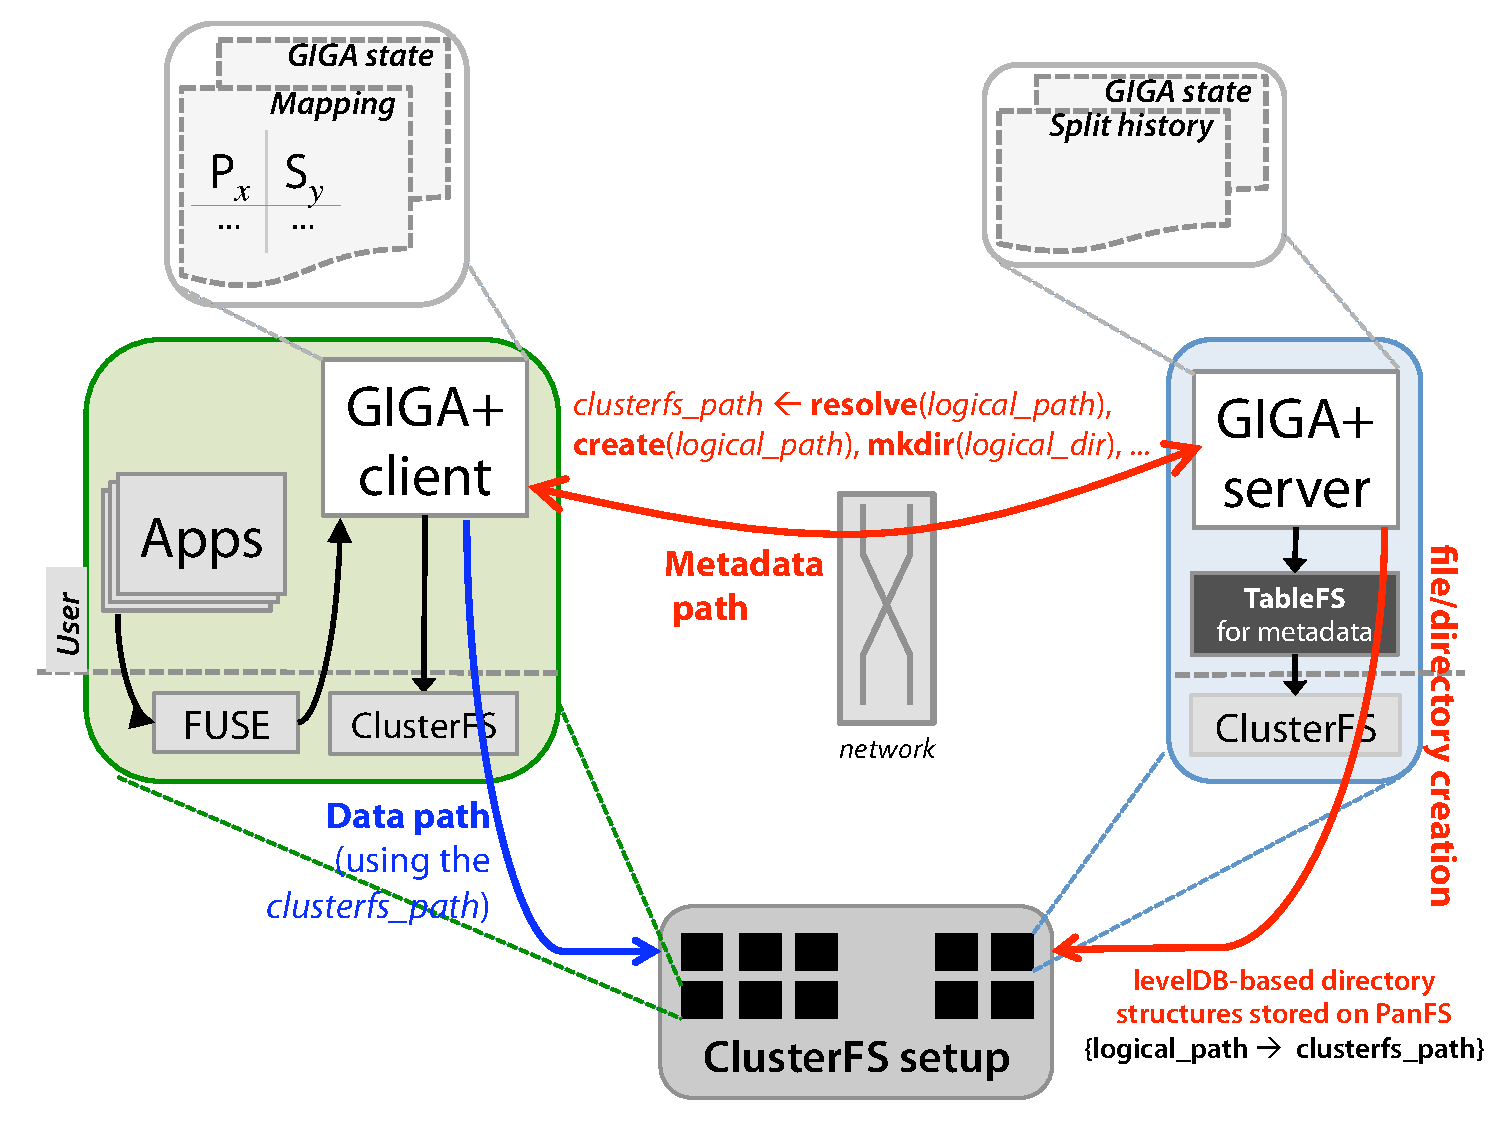
\includegraphics[scale=0.3]{./figs/giga-impl-leveldb-clusterfs}}
\caption{\normalsize
%\textbf{Proposed design.}
Design of our scalable metadata middleware that integrates a distributed metadata indexing
technique with a tabular metadata-optimized on-disk layout on each server and
layers on existing cluster file systems. 
%Our approach for a scalable metadata service integrates two components: a highly 
%parallel and load-balanced indexing technique (called \giga{} \cite{GIGA}) to 
%partition
%metadata over multiple servers and an optimized metadata representation (called
%\tfs{} \cite{TableFS}) on each server. 
%Our approach aims to layer this integrated solution on top of existing cluster file 
%system deployments. 
}
\vspace{10pt}
\hrule 
\label{fig:design}
\end{figure}       %% END_FIGURE

Figure \ref{fig:design} shows the architecture of our scalable metadata
service that is designed to be layered on existing deployments of cluster file
systems. Our approach uses a client-server architecture and has three components: 
unmodified applications running on clients, the \giga{} directory indexing service 
on clients and servers, and the \ldb{}-based persistent metadata representation 
managed by the server.
Applications interact with our middleware using the VFS interface exposed
through the FUSE user-level file system \cite{fuse}.
All metadata requests, such as \texttt{create()}, \texttt{mkdir()} and
\texttt{open()}, are handled through the \giga indexing modules that address
the request to the appropriate server.
Each indexing server manages its local \ldb instance to store and access all
metadata information. This \ldb instance stores flat files (in its special
format) containing changes in metadata. 
Once the client receives the relevant metadata back from the server, our
middleware allows clients to access the actual file contents directly through
the cluster file system.

Using \giga{} and \ldb{} enables us to tackle two key challenges: highly 
concurrent metadata distribution for ingest-intensive parallel applications
such as checkpointing \cite{PLFS} and 
optimized metadata representation that stores all file system
metadata in structured, indexed files manages by existing cluster file system
deployments \cite{LevelDB}. 

Remainder of this section describes more details of our approach. 
Section \ref{design.giga} presents a primer on how \giga{} distributes 
metadata. 
Section \ref{design.tablefs} shows how \ldb{} stores all file system metadata
using a single on-disk structure on each server. 
Section \ref{design.integration} describes the challenges in effectively
integrating \giga{} and \ldb{} to work with existing cluster file systems.

\subsection{Scalable partitioning using \giga{}}
\label{design.giga}
%\section*{\giga{} indexing approach}
%\label{indexing}

\giga{} is a distributed hash-based indexing technique that incrementally
divides each directory into multiple partitions that are spread over multiple 
servers \citep{GIGA11}.
Each filename stored in a directory entry is hashed and mapped to a partition 
using an index. 
\giga{} selects a hash partition such that for any distribution of unique filenames, the hash values of 
these filenames will be uniformly distributed in the hash space.
In addition to load-balanced distribution, \giga{} also grows the directory
index incrementally, i.e. all directories start small on a single server, and
then expand to more servers as they grow in size. 

The core idea behind \giga{} is parallel splitting: each server splits 
without system-wide serialization or synchronization.
Every server makes a local decision, without coordinating with other servers, 
about when to split a partition. 
Such uncoordinated growth causes \giga{} servers to have a partial view of the
entire index; there is no central server that holds the global view of the 
partition-to-server mapping.
Each server knows about the partition it stores and the 
identity of another server that knows more about each ``child'' partition resulting
from a prior split by this server. 
This information is known as the per-server split history of its partitions.
The full \giga{} index is a transitive closure of the split history on each
server and represents the lineage of directory partitioning.

The full index (and split history) is also not maintained synchronously by any client.
\giga{} clients can enumerate the partitions of a directory by traversing 
its split histories starting with the first partition that was created during
\texttt{mkdir}.
However, such a full index that is cached by a client may be stale at
any time, particularly for rapidly mutating directories.
\giga{} allows clients to keep using the stale mapping information and
receiving mapping updates from servers. 
More discussion on the cost-benefit of using
inconsistent mapping state is not relevant to this work and can be found in
prior \giga{} literature \citep{GIGA11, GIGA07}. 

%%%%%%%%%%%


\begin{comment}
\textbf{Tolerating inconsistent mapping at clients -- }
%\subsection*{Tolerating inconsistent mapping at clients}
%\label{indexing:inconsistency}
Clients seeking a specific filename find the appropriate partition by probing 
servers, possibly incorrectly, based on their cached index.
To construct this index, a client must have resolved the directory's parent
directory entry which contains a cluster-wide i-node identifying the server and
partition for the zeroth partition $P_0$.
Partition $P_0$ may be the appropriate partition for the sought filename, or it
may not because of a previous partition split that the client has not yet
learned about. 
An ``incorrectly'' addressed server detects the addressing error by recomputing 
the partition identifier by re-hashing the filename.
If this hashed filename does not belong in the partition it has,
this server sends a split history update to the client.
The client updates its cached version of the global index and 
retries the original request.

The drawback of allowing inconsistent indices is that clients may need 
additional probes before addressing requests to the correct server.
The required number of incorrect probes depends on the client request 
rate and the directory mutation rate (rate of splitting partitions).
It is conceivable that a client with an empty index may send O$(log(N_p))$ 
incorrect probes, where $N_p$ is the 
number of partitions, but \giga{}'s split history updates makes this many
incorrect probes unlikely.
Each update sends the split histories of all partitions that reside on a
given server, filling all gaps in the client index known to this server and
causing client indices to catch up quickly.
Moreover, after a directory stops splitting partitions, clients soon after will 
no longer incur any addressing errors.
%\giga{}'s eventual consistency for cached indices is different from LH*'s
%eventual consistency because the latter's idea of independent splitting (called
%pre-splitting) suffers addressing errors even when the index
%stops mutating \citep{lh*:litwin96}. 

\textbf{Key performance insights -- }
Detailed analysis of the scalability and performance of \giga{} studies several
tradeoffs \citep{giga}; the observations that are within the scope of this work
include the load-balancing and incremental growth strategy.


%%%%%%%%%%%
\subsection*{On-line server additions}
\label{indexing.reconfig}

%This section describes how \giga{} adapts to the addition of servers in a 
%running directory service.
%\footnote{Server removal (i.e., decommissioned, not 
%failed and later replaced) is not as
%important for high performance systems so we leave it to be done by user-level
%data copy tools.}

\begin{figure}[t]
\centerline{\includegraphics[scale=0.35]{../common/figures/giga-serveradd}}
\vspace{-10pt}
\caption{\small
\textbf{\giga{} server additions.}
By changing the partition-to-server mapping from round-robin on the original 
server set to sequential on the newly added servers, \giga{} can minimize the amount
of data migrated (shown by arrows indicating splits).
}
\label{fig:giga-adding}
%\vspace{10pt}
%\hrule depth 0.5pt
\end{figure}

When new servers are added to an existing configuration, the system is
immediately no longer load balanced, and it 
should re-balance itself by migrating a minimal number of directory entries
from all existing servers equally. 
Using the round-robin partition-to-server mapping, shown in Figure 
\ref{fig:giga-indexing}, a naive server addition scheme would require 
re-mapping almost all directory entries whenever a new server is added.

\giga{} avoids re-mapping all directory entries on addition of servers by 
differentiating
the partition-to-server mapping for initial directory growth from the mapping
for additional servers.
For additional servers, \giga{} does not use the round-robin partition-to-server
map (shown in Figure \ref{fig:giga-indexing}) and instead 
maps all future partitions to the new servers in a ``sequential manner''.
The benefit of round-robin mapping is faster exploitation of parallelism
when a directory is small and growing, while a sequential mapping for the tail
set of partitions does not disturb previously mapped partitions more than is 
mandatory for load balancing.
Figure \ref{fig:giga-adding} shows an example where the original configuration
has 5 servers with 3 partitions each, and partitions $P_0$ to $P_{14}$ use a 
round-robin rule (for $P_i$, server is $i$ \texttt{mod} $N$, where $N$ is 
number of servers).
After the addition of two servers, the six new partitions $P_{15}$-$P_{20}$
will be mapped to servers using the new mapping rule: $i$ \texttt{div} $M$, 
where $M$ is the number of partitions per server (e.g., 3 partitions/server).

In \giga{} even the number of servers can be stale at servers and clients. 
The arrival of a new server and its order in the global server list is declared
by the cluster file system's configuration management protocol, such as
Zookeeper for HDFS \citep{zookeeper:hunt10}, leading to each existing server
eventually noticing the new server.
Once it knows about new servers, an existing server can inspect its partitions
for those that have sufficient directory entries to warrant splitting and would
split to a newly added server.
The normal \giga{} splitting mechanism kicks in to migrate only directory
entries that belong on the new servers.
The order in which an existing server inspects partitions can be entirely
driven by client references to partitions, biasing migration in favor of active
directories.
Or based on an administrator control, it can also be driven by a background 
traversal of a list of partitions whose size exceeds the splitting threshold. 

\end{comment}


\subsection{Metadata layout using \ldb{}}
\label{design.tablefs}
%\section{Table-based local store}

\tfs \cite{TableFS} is a stacked local file system, 
which uses another local file system as an object store 
and organizes all metadata into a single sparse table backed on-disk 
using a Log-Structured Merge (LSM) tree \cite{ONeil1996}, LevelDB\cite{LevelDB} in our experiments.
By using an LSM tree, TableFS ensures metadata is written to disk in large, non-overwrite, sorted and indexed logs.
The detailed design of  \tfs and LevelDB are explained as the follows.

\subsubsection*{LevelDB and LSM Tree}
Inspired by a simpler structure in BigTable\citep{BigTable}, 
LevelDB \citep{LevelDB} is an open-source key-value storage library
that features an Log-Structured Merge (LSM) Tree \citep{ONeil1996} for on-disk storage.
It provides simple APIs such as GET, PUT, DELETE and SCAN.
In a simple understanding of an LSM tree, an in memory buffer cache delays 
writing new and changed entries until it has a significant amount of change to record on disk. 

\begin{figure}[!ht]
\centering
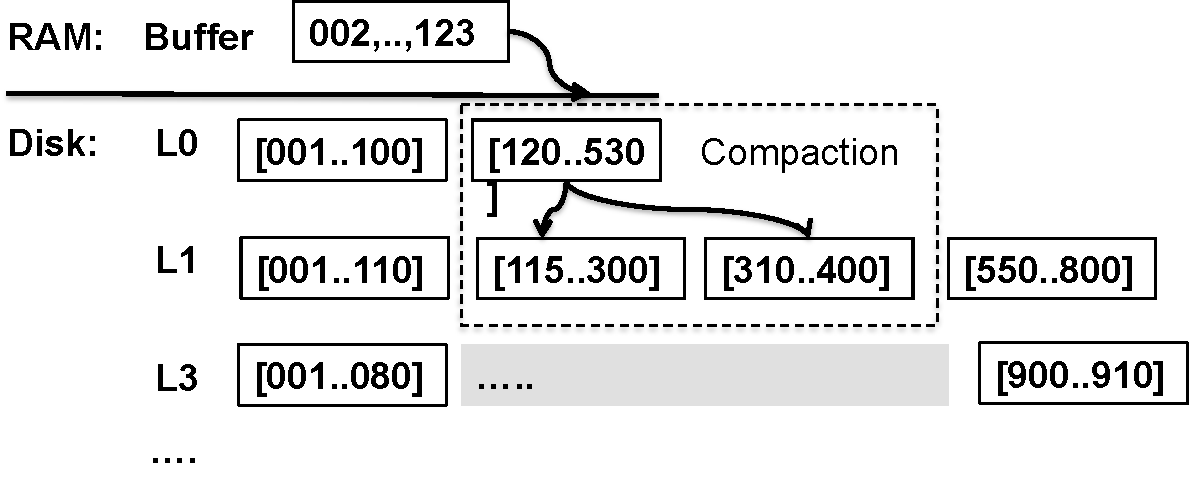
\includegraphics[scale=0.4]{figs/leveldb}
\caption{LevelDB represents data on disk in multiple SSTables that store sorted key-value pairs.}
\label{fig:leveldb}
\end{figure}


In LevelDB, by default, a set of changes are spilled to disk when the total size of modified entries exceeds 4 MB.  When a spill is triggered, called a minor compaction, the changed entries are sorted, indexed and written to disk in a format called an SSTable\citep{BigTable}.  These entries may then be discarded by the in memory buffer and can be reloaded by searching each SSTable on disk, possibly stopping when the first match occurs if the SSTables are searched most recent to oldest.  The number of SSTables that need to be searched can be reduced by maintaining a Bloom filter\citep{bloomfilter} on each, but with time the cost of finding a record not in memory increases.  Major compaction, or simply ``compaction", is the process of combining multiple SSTables into a smaller number of SSTables by merge sort. 

As illustrated in Figure \ref{fig:leveldb}, LevelDB extends this simple approach to further reduce read costs by dividing SSTables into sets, or levels.
The 0-th level of SSTables may contain entries with any key value, based on what was in memory at the time of its spill.
The higher levels of LevelDB's SSTables are the results of compacting SSTables from their own or lower levels.
In these higher levels, LevelDB maintains the following invariant: the key range spanning each SSTable is disjoint from the key range of all other SSTables at that level.
So querying for an entry in the higher levels only need read at most one SSTable in each level.
LevelDB also sizes each of the higher levels differentially:  all SSTables have the same maximum size and the sum of the sizes of all SSTables at level $L$ will not exceed $10^L$ MB.
This ensures that the number of level grows logarithmically with increasing numbers of entries.

\subsubsection*{Table Schema} 

\tfs's metadata store aggregates directory entries, 
inode attributes into one LevelDB table with a row for each file / directory.
To link together the hierarchical structure of the user's namespace,
the rows of the table are ordered by a 224-bit key consisting of 
the 64-bit inode number of a file's parent directory 
and a 160-bit SHA-1 hash value of its filename string (final component of its pathname).
The value of a row contains the file's full name and inode attributes,
such as inode number, ownership, access mode, file size, timestamps (\textit{struct stat} in Linux),
and a symoblic link that contains the actual path of the file object in the object store.
Figure \ref{fig:schema} shows an example of storing a sample file system's metadata into one LevelDB table.

\begin{figure}[!ht]
\centering
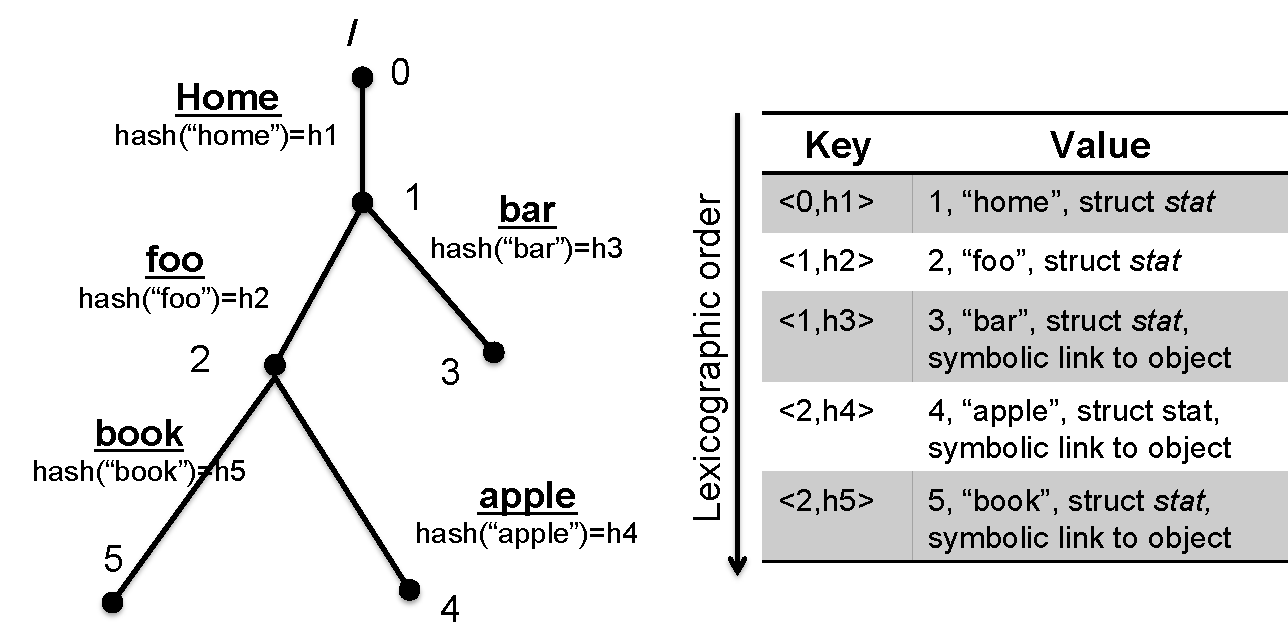
\includegraphics[scale=0.35]{figs/schema}
\caption{An example illustrates table schema used by \tfs's metadata store.}
\label{fig:schema}
\end{figure}

All the entries in the same directory have rows that 
share the same first 64 bits in their the table's key.
For $readdir$ operations, once the inode number
of the target directory has been retrieved, 
a scan sequentially lists all entries having 
the directory's inode number as the first 64 bits of their table's key. 
To resolve a single pathname, \tfs starts searching from the root inode, 
which has a well-known global inode number $(0)$.
Traversing the user's directory tree
involves constructing a search key by concatenating the inode 
number of current directory with the hash of
next component name in the pathname.


\subsection{Integrating \giga{} and \ldb{}}
\label{design.integration}

To effectively integrate the \giga{} distribution mechanism with the
\ldb{}-based metadata representation, we tackled several challenges. 

~\\
\textbf{Metadata representation -- }
\ldb{} stores all metadata including \giga{} hash
partitions for directories, entries in each hash partition, and other
bootstrapping information such as root entry and \giga{} configuration state.
The general schema used to store all file is:
%\texttt{\{key\} --> \{value\}} format:

\begin{verbatim}
    <KEY>         -->     <VALUE> 

{parentDirID,         {attr(dirEntry),
 gigaPartitionID, -->  symlink,
 hash(dirEntry)}       gigaMetaState}
\end{verbatim}

The main difference from the \ldb{} schema described in Section
\ref{design.tablefs} is the addition of two \giga specific fields: 
\texttt{gigaPartitionID} to identify a
\giga{} hash partition and \texttt{gigaMetaState} to store the
hash partition related mapping information. These \giga{} related fields are 
used only if large directories are distributed over multiple metadata servers.\footnote{
Since we already store the \texttt{hash} of the directory entry, we can use the
hash-values to identify hash partitions if we chose to use the same hash
function for both \giga and \ldb keys. This optimization can eliminate the
need for \texttt{gigaPartitionID} in the schema.} 

~\\
\textbf{Partition splitting -- }
Each \giga{} hash partition and its directory entries are stored in sorted
SSTable files in a local \ldb{} instance. 
Recall that each \giga{} server process splits a hash partition $P$ on 
overflow and creates another hash partition $P'$ which is managed by a 
different server; this split involves migrating approximately half the entries 
from old partition $P$ to the new hash partition $P'$ on another server during
which the key range in write locked.
We explored several ways to perform this cross-server partition split.

A simple approach to splitting would be to perform a \ldb range scan on 
partition $P$ and deleting about half the results (corresponding to the keys
that are migrated to the new partition) from $P$. 
All entries that need to be moved to the new partition $P'$ are batched
together and sent in an RPC message to the server that will manage partition 
$P'$.
The recipient server inserts each key in the batch in its own \ldb{}
instance. While the simplicity of this approach makes it attractive, we would
like a faster technique that to reduce the time the range is write locked. 

The immutability of \ldb SSTables makes such a fast bulk insert possible -- an
SSTable can be added to Level 0 without its data being pushed through the
write-ahead log and minor compaction process.
To take advantage of this opportunity, we extended \ldb{}
to support a three-phase split operation. 
First, the split initiator performs a range scan on its \ldb{} instance to find all
entries in the hash-range that needs to be moved to another server. The results
of this scan are written in a \ldb{}-specific SSTable format to file in the
underlying cluster file system. 
In the second step, the split initiator notifies the split receiver about
the new \ldb{}-format file in a much smaller RPC message.
The split receiver then bulk inserts the file into the \ldb{} tree structure 
instead of iteratively inserting one key at a time.
The final step is a clean-up and commit phase: after the receiver completes the 
bulk insert operation, it notifies the 
initiator, who then deletes the migrated hash-range from its LevelDB instance
and unlocks the range.%\footnote{
%This three-phase split can be refined even further: \ldb{} can use symbolic links 
%to these split files without explicitly copying the files through shared
%storage. Because the current release of \ldb{} does not have support for links, we 
%left this optimization for future work. 
%}

~\\
\textbf{Decoupled data and metadata path -- }
All metadata operations go through the \giga{} server; however, following the
same path for data operations would incur an unnecessary performance penalty 
of shipping data over the network on extra time. 
This penalty can be significant in HPC use-cases where files can easily be  
gigabytes to terabytes in size.

To avoid this penalty our middleware is designed to perform all
data-path operations directly through the cluster file system module in client
machine. 
Figure \ref{fig:design} illustrates this data path (in BLUE color).
Once the client completes a
lookup on a desired file name, it gets back a symbolic link to the physical
path in the cluster file system. All subsequent access using this symbolic
link force the client operating system to resolve this link into the cluster
file system.
While the file is open, its attributes may change relative to \ldb's per-open
copy of the attributes. \giga will capture these changes on file close on the
metadata path.

%\subsubsection*{Other challenges.}


\section{Evaluation}

\begin{figure}[t]  %%%%%%%%%%%%%%%%%%%%%%%
\centerline{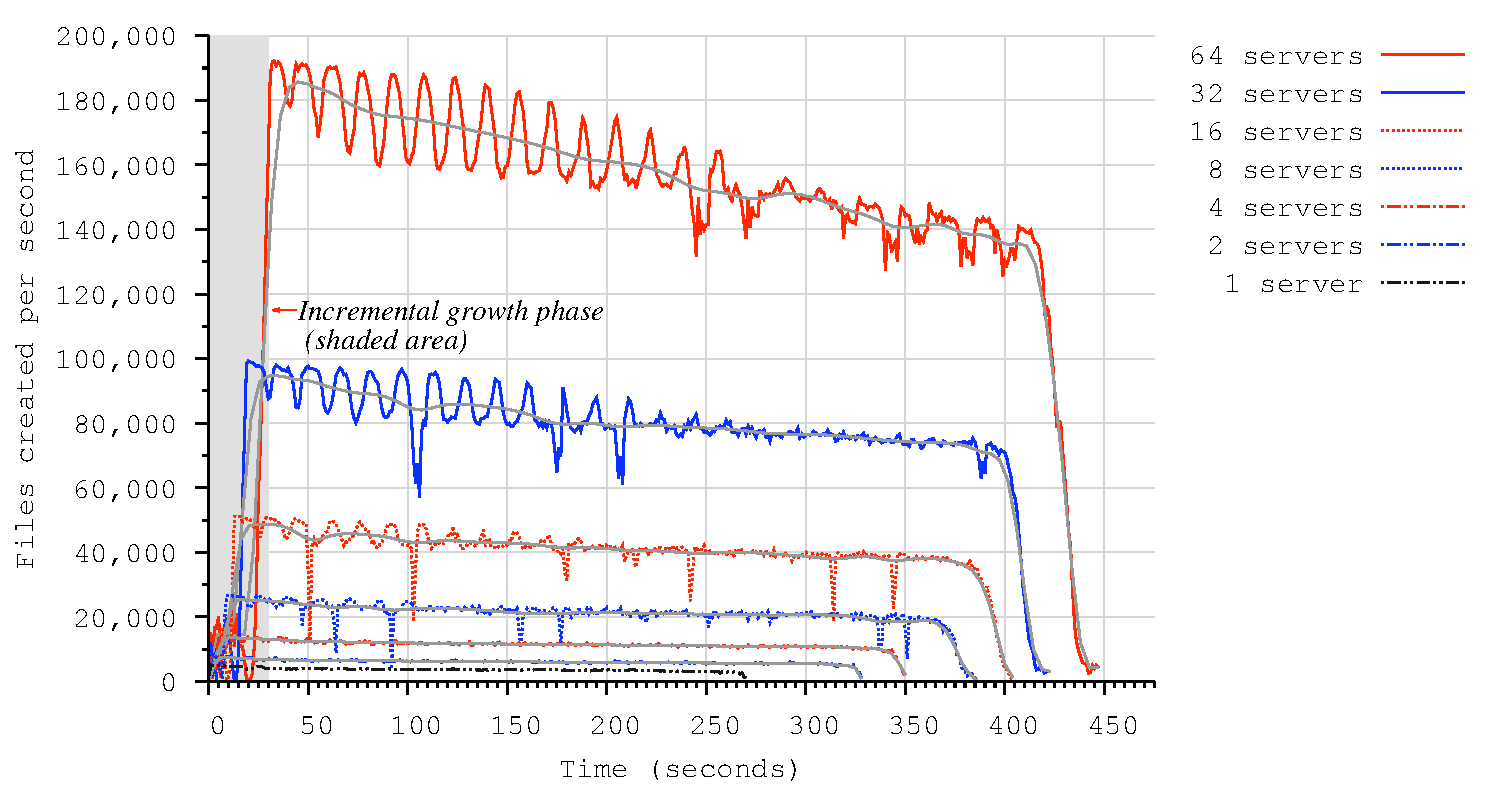
\includegraphics[scale=0.33]{./figs/ldb_insertrate}}
\caption{
\textbf{Scale-out performance on an on-disk LevelDB backend.}
{\small
\giga{} using a disk-based LevelDB backend shows promising scalability
up to 64 servers. However the interaction between LevelDB's compaction policies and 
the Linux Ext3's implementation policies causes periodic throughput variance
that degrades as the the number of directory entries in each LevelDB
increases. \textit{Note that the solid lines in each configuration are Bezier
curves to smooth the variability.}
}
}
\vspace{15pt}
\hrule 
\label{graph:ldb-scaling}
\end{figure}       %%%%%%%%%%%%%%%%%%%%%%%

Figure \ref{graph:ldb-scaling} shows the instantaneous throughput during the 
\textit{concurrent create} workload in a strong scaling experiment, i.e.
creating 1 million files per server and reaching up to 64 million files in the
64 server configuration.
The main result in this figure is that as the number of servers doubles the
throughput of the system also scales up. With 64 servers, \giga{} can achieve a
peak throughput of about 190,000 file creates per second. The system delivers
this peak performance after the directory workload has been spread among all
servers.
Before reaching steady-state, the throughput grows gradually due to the splitting
policies adopted by \giga{}. We take a closer look at this incremental growth in
the next chapter.

Another key observation in Figure \ref{graph:ldb-scaling} is that the system is
unable to sustain the steady-state peak throughput: in fact, in large setups
with 8 or more servers, the peak throughput drops by as much as 25\% (in case
of the 64-server setup). 
This happens for two reasons, both related to the policies and behavior of
LevelDB.

\begin{figure}[t]  %%%%%%%%%%%%%%%%%%%%%%%
\centerline{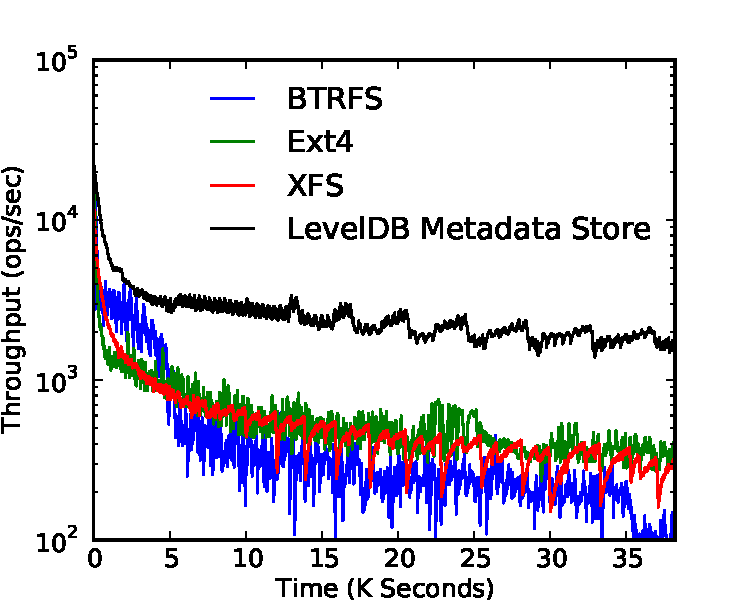
\includegraphics[scale=0.45]{./figs/ldb_insertrate_onenode}}
\caption{
\textbf{Single-node LevelDB performance compared to three Linux filesystems.}
{\small
A one-server configuration with LevelDB backend shows the performance of creating 100 million zero-length files.
We only graph the time until LevelDB finished inserting all 100 million zero-length files, 
because the other file systems were much slower. LevelDB is 10X faster than the other tested file systems.
The veritical axis is in a log scale.
}
}
\vspace{15pt}
\hrule 
\label{graph:ldb-singlenode}
\end{figure}       %%%%%%%%%%%%%%%%%%%%%%%

The first reason is periodic \textit{compactions} in LevelDB that create
ordered files 
by periodically sorting the in-memory log and writing them to separate files 
on-disk. If there are pre-existing files from previous compactions, LevelDB merges 
these old files with newly arrived in-memory logs to write out most recent sorted 
sequential files. These compactions cause both read and write disk I/O:
existing sorted files are read into memory and newly merged files are written
back to disks. Figure \ref{graph:ldb-singlenode} shows the variability in insert
throughput of a single node instance of LevelDB-based backend. This figure
shows that periodic background compactions happen during the entire experiment
which causes the throughput to drop steadily -- the overall throughput drop is
more than 35\% of the peak throughput.
In Figure \ref{graph:ldb-scaling}, the throughput drop is much higher in
aggregate but is about the same fraction as the single-node degradation.
This is expected because each LevelDB instance performs these compactions, and 
because each \giga{} server handles a uniform load, all LevelDB instances are busy
performing compactions.  

The second reason for the degrading saw-tooth behavior in Figure
\ref{graph:ldb-scaling} is due to the choice of LevelDB key used by \tfs{}.
Recall that \tfs{} uses a combination of the file name, the parent directory's
unique identifier and the hash value of the file name as the key. 
The hash value of the file name causes an interesting tradeoff: it simplifies
LevelDB's split optimizations but it makes LevelDB's compactions more I/O
intensive.
Because the hash values are uniformly random, even two lexicographically
similar file names in the same parent directory will have random, and
lexicographically very different, hash values.
This makes the entire LevelDB key lexicographically different which causes
LevelDB to read more files during compactions.

To confirm our hypothesis, we compared the variability in LevelDB's insert
throughput for different keys.
Figure "comingInTheFuture" will hopefully how this tradeoff (XXX).
%XXX: function of different keys and values 


\section{Future challenges}
\label{futurework}

Before our work can be useful in real HPC deployments, we need to address
several challenges.

First, we plan to layer our middleware on top of a real cluster file system
such as Panasas PanFS \citep{panfs:welch08} or PVFS \citep{pvfs:www}. This will
allow us to inherit the data path scalability when accessing the flat SSTable
files of \ldb that are stored on the data servers. We also plan to explore how
we can effectively leverage the fault tolerance mechanisms and system
configuration tools already present in the cluster file systems.

Second, we would like to minimize the FUSE overheads of accessing the file.
Even after the application gets a symbolic link pointing to the physical
location of the file, our current prototype will rely of FUSE and VFS to
dereference the symbolic link. Ideally, we would like to avoid this FUSE
interposition by changing the FUSE kernel module to support distributed file
system file handles. 

Third, we are exploring several optimizations to minimize the background
compaction operations triggered by \ldb. These compactions are a necessary
evil: they speed up future reads and scans, while affecting any foreground
operations that happen during these background operations. {\bf TODO: what else?}

\section{Summary}
\label{summary}

Modern cluster file systems provide highly scalable I/O bandwidth along the
data path by enabling highly parallel access to file data.
Unfortunately metadata scaling is lacking behind data scaling; we propose an
idea to re-use 

%inhertts data bandwidth and adds the metadata bandwidth scaling

%split and migrate without moving the underlying objects





%\pagebreak
%\newpage

\vspace{11pt}
\hrule{}
%\small
%\textbf{Acknowledgements.}

\vspace{11pt}
%%%%%%%%%%%%%%%%%%%%%%%%%%%%%%%%%%%%%%%%%%%%%%%%%%%%%%%%%%%%%%%%%%%%%%%%%%%%%%
%%%%%% Add bibliography 
%%%%%%
\setlength{\bibsep}{3pt}
%\small
\footnotesize
\bibliographystyle{acm}
%\bibliographystyle{myAuthorDate}
\bibliography{reference}
%\bibliography{../pubs}

\end{document}

%%%%%%%%%%%%%%%%%%%%%%%%%%%%%%%%%%%%%%%%%%%%%%%%%%%%%%%%%%%%%%%%%%%%%%%%%%%%%%
